\documentclass[a4paper,11pt,twoside,openright]{scrbook}

\usepackage{swThesis}
\usepackage{amsmath}
\usepackage{lipsum}
\usepackage{microtype}
\usepackage{booktabs}
\usepackage{standalone}
\usepackage{epigraph}  % For dedication and quote
\usepackage{bibentry}  % Allow full citations in text

\usepackage{import}
\standalonetrue

\bibliography{bibliography}

% Figures
\graphicspath{{../figs/}}

\begin{document}

\chapter{Cell morphology can be used to predict compound mechanism-of-action} \label{chapter:moa}

\section{Introduction}
Cellular morphology is influenced by multiple intrinsic and extrinsic factors acting on a cell, and striking changes in morphology are observed when cells are exposed to biologically active small molecules.
This compound-induced alteration in morphology is a manifestation of various perturbed cellular processes, and we can hypothesise that compounds with similar MoA which act upon the same signalling pathways will produce comparable phenotypes, and that cell morphology can, in turn, be used to predict compound MoA.

In 2010 Caie \textit{et al.} generated, as part of a larger study, an image dataset consisting of MCF7 breast cancer cells treated with 113 small molecules grouped into 12 mechanistic classes, these cells were then fixed, labelled and imaged in three fluorescent channels\cite{Caie2010}.
This dataset (also known as BBBC021) has become widely used as a benchmark in the field for MoA classification tasks, with multiple publications using the images to compare machine learning and data pre-processing approaches. \cite{Ljosa2013a,Singh2014a,Pawlowski2016,Ando2017}
Whilst this is important work, it has led to the situation whereby the vast majority of studies in this field have based their work on a single dataset generated with one cell-line.

One of the issues associated with phenotypic screening when used in a drug discovery setting is target deconvolution.
Once a compound has been identified which results in a desirable phenotype in a disease-relevant assay it is common to want to know which molecular pathways the hit compound is acting upon.
While target deconvolution is a complex and difficult task, image-based morphological profiling represents one option similar to transcriptional profiling that can match and unknown compound to the nearest similar annotated compound in a dataset to inform compound MoA, while at the same time being far cheaper than the transcriptional methods such as LINCS1000 \cite{Duan2014}.


\subsection{Machine learning methods to classify compound MoA}
Predicting compound MoA from phenotypic data is a classification task.
This type of machine learning problem is well researched, and there are several models appropriate for our labelled data.
As the raw data is in the form of images, it can be approached as an image classification task, a problem in the field receiving lots of attention due to recent theoretical and technological breakthroughs. %citations?
Whereas a more classical approach would be to extract morphological information from the images, generating a multivariate dataset from the images, and training a classifier on these morphological features.

To develop and validate a machine learning model the dataset has to be split into training, validation and test sets.
This is because overfitting is a common problem in machine learning, whereby the model is trained and accurately predicts labels on one dataset, but performs poorly when applied to new data on which is was not trained.
Most classification models will overfit to some degree, typically performing better on the training dataset than any other subsequent examples, but the challenge is to limit this overfitting, and also to ensure that the data used to report accuracy measures has not been used in any way to train or validate the model.


% comparison of machine learning and data pre-processing methods to predict MOA
% from morphological data

% description / background of each method
% pros / cons of each
% results
% conclusion of comparison

\subsection{Ensemble of decision trees trained on extracted morphological features}
A decision tree is a very simple method that can be used for both regression and classification.
The method works by repeatedly dividing the decision space using binary rules on the feature values until a terminal node containing a classification label is reached (figure \ref{figure:decision_tree}).
Simple decision trees like those shown in figure \ref{figure:decision_tree} perform relatively poorly on all but the simplest of classification problems.
However, by aggregating many decision trees and their predictions we can create more accurate and robust models in a practice known as ensemble learning. \cite{Opitz1999}
Bagging \cite{Breiman1996} and Boosting \cite{Freund1996} are two popular methods for constructing ensembles of decision trees.
As combining the output of several decision trees is useful only if there is a disagreement among them, these two methods both attempt to solve the same problem of generating a set of correct decision tress, that still disagree with one another as much as possible on incorrect predictions.


\begin{figure}
    \captionsetup{width=0.8\textwidth}
    \caption[Diagram of a simple decision tree]{\textbf{(A)} An example of a simple mock decision tree to classify compound mechanism of action based on morphological features. \textbf{(B)} Depiction of decision space as divided by the decision tree model. Shaded areas show how new input data will be classified based on the decision rules (dotted lines).}
    \input{figs/ch2DecisionTree.pdf_tex}
    \label{figure:decision_tree}
\end{figure}

% using extracted morphological features
Decision tree methods work best with multivariate tabular data, with well defined features describing each observation, this is in contrast to image data which consists of 2D arrays of pixel intensities.
Therefore, in order to train such a model, cellular morphology needs to be quantified by measuring cellular features.
This is a common task with multiple software packages available, which follow two main steps: (1) Segment objects from the background. Objects may be sub-cellular structures or whole-cell masks (2) Measure various attributes from the object, this is typically based on size, shape and intensity.
Cellprofiler \cite{Carpenter2006} was chosen primarily due to the high configurability and the permissive license enabling large-scale distributed processing on compute clusters in order to reduce the image analysis time.
The images captured on the ImageXpress were analysed using Cellprofiler, quantifying approximately 400 morphological features.
The datasets produced by the Cellprofiler analysis contained morphological measurements on an individual cell level.
Although we can train a model on single cell data we are not interesting in classifying morphologies of single cells, but rather classifying an image or a collection of images that represent a compound treatment, this therefore allows several approaches to structuring the training data:

\begin{enumerate}
    \item Train and test on median profiles.
    \item Train on single cell data, test on image or well median profiles.
    \item Train on single cell data, test on single cell data and classify the parent image as the most commonly predicted class of cell in that image.
    \item Train on median profiles of boostrapped single cell samples within an image, and test on median profiles.
\end{enumerate}


% image averages, vs single cell data and consensus classification.
    % comparison of both.


\subsection{Convolutional neural networks trained on pixel data}
Artificial neural networks (ANNs) are becoming increasingly common in a wide range of machine learning tasks.
Although many of the theories underpinning ANNs are decades old, \cite{Rosenblatt1958} they have only recently achieved widespread practical use due to improved methods for training \cite{Rumelhart1986} and the availability of more computing power allowing the use of more complex models.
ANNs are (very) loosely inspired by the structure of biological brains, with interconnected neurons passing signals through layers onto subsequent neurons forming a chain with the output of one neuron becoming the input for the next neuron.
In between neurons, the signals can be altered by multiplying the value by a weight ($W$), it is through adjusting these individual weights that ANNs optimise their performance for a particular task, similar to how long-term potentiation is used to strengthen synaptic connections in biological brains.
When a signal reaches a neuron, it is combined via a weighted sum with all the other inputs from other connected neurons and passed through an activation function.
This activation function -- similar to an action potential in neurons -- determines the output of the neuron for the given aggregated input, which is then passed as new inputs onto subsequent neurons and so on, however, in contrast to an all-or-nothing output of an action potential there are several types of activation functions used in ANNs, most of which have a graded output (figure \ref{figure:neuron_relu}B).

\begin{figure}
    \captionsetup{width=0.9\textwidth}
    \caption[Diagram neural network neuron and activation function.]{\textbf{(A)} A representation of a single connected neuron in an ANN, the input value to the neuron is multiplied by the weight ($W_1$), before being passed through the activation function $R$, the output of which is then multiplied by $W_2$, and passed as the input to the next neuron. \textbf{(B)} A neuron with multiple inputs and outputs, typical of those in a hidden layer. The activation function acts on the weighted sum of all inputs, and returns a single output value which is when directed to all connected neurons in the next layer. Where $W_i$ is the weight of \textsf{input}$_i$. \textbf{(C)} A common activation function also known as a rectifier, in this example a rectified linear unit (ReLU), in the inputs ($x$) is transformed and passed as output. So $f(x)$ can be viewed as the output for a given value of $x$.}
    \label{figure:neuron_relu}
\input{figs/ch2NeuralNetworkNode2.pdf_tex}
\end{figure}

The neurons in an ANN are typically arranged in several layers: an input layer; one or more hidden layers; and a final output layer (figure \ref{figure:nn_layers}).
With each layer, the network transforms the data into a new representation, through training the network these representations make the data easier to classify.
In the final layer, the data is ultimately represented in a way which makes a single output neuron activate more strongly than the other neurons in that layer, and so the data is ultimately transformed into a single value -- the index of the active neuron which corresponds to a particular class.
A new ANN is initialised with random weights, to train a neural network these weights are adjusted by feeding in labelled data and adjusting weights in order to minimise classification errors through a process known as backpropagation.\cite{Rumelhart1986}




\begin{figure}
\fcapsideleft
{
    \caption[Representation of a simple ANN]{Representation of a simple 3-layer ANN with a single fully connected hidden layer, three input neurons and three output neurons. $W$ denotes a weighted connection between an input neuron and a hidden-layer neuron, with all connections between neurons having an associated adjustable weight. A network such as this would take a vector of three numbers as input, and would be capable of predicting three classes from the output layer of three neurons depending on the activation strengths of the neurons in the final output layer.}
} {
    \input{figs/ch2NeuralNetworkLayers.pdf_tex}
    \label{figure:nn_layers}
}
\end{figure}

%convolution part of convolution neural networks
The convolution aspect of convolutional neural networks plays an important role when working with image data.
Two-dimensional convolutions are widely used in image processing -- blurring, sharpening and edge detection are all common operations which use this operation.
They work by mapping a kernel -- a smaller matrix of values -- across a larger matrix, thereby using information from a small region of pixels in their transformation of each individual pixel.
This lends itself well to ANNs, as a pixel value in isolation is less informative than a pixel value in the context of the neighbouring values.
Depending on the size and the values within the kernel, the transformations highlight different features within an image.
Two dimensional convolutions are used in ANNs by starting with many randomly initialised kernels, and updating the kernel values through training in order to best highlight features which prove useful for accurately predicting classes.
Using a single convolutional layer highlights simple features in an image such as edges and speckles, by combining several convolutional layers more complex features are highlighted through combinations of these simple features.
These convolved images are then flattened into a one-dimensional vector which is used as an input in a fully connected ANN such as that depicted in figure \ref{figure:nn_layers}.


\subsection{Chapter aims}
%TODO: aims of the chapter
The aims of this chapter are to assess how well machine learning models to predict compound MoA transfer across morphologically distinct cell lines.
This is of interest as the ability to predict the MoA of unannotated compounds on a new cell-line with a pre-trained model without the requirement of re-screening an annotated compound library would save time and money.

%TODO: need some intro into the tasks, the mechanistic classes.
The compound library used in this work consist of 24 annotated compounds with well defined MoAs.



\section{Results}

\subsection{CNN predictions are improved using sub-images}

The images generated by the ImageXpress microscope with zero binning are 2160$\times$2160 pixel tiff files, with a bit-depth of 16, whilst these image properties are common in microscopy, they are extreme for current CNN implementations.
Most image classification tasks involving CNN's use 8-bit images in the region of 300 by 300 pixels, relatively small images are used as the convolutional layers of deep CNN's generate many thousands of matrices, and using smaller input images drastically reduces the computing resources and time required to train such classifiers.

This presents the issue of how to reduce the 2160$\times$2160 images into small images, one option is to downscale the entire image using bi-linear or bi-cubic interpolation, while a second option is to chop the original image up into smaller sub-images (figure \ref{figure:image_chopping}).
Downsizing the original image by simple scaling has a few potential problems which make it unsuitable for this particular task:
    many of the finer-grained cell morphologies such as mitochondria and endoplasmic reticulum distribution will be lost due to the reduction in image resolution;
    in addition, it was found that whole well images are susceptible to over-fitting as the classifier learned biologically irrelevant features such as the locations of cells within an image, which although should be random might have some spurious association with particular class labels.
When chopping images into sub-images the most simple and commonly used method is to chop each image into an evenly spaced grid, whilst this is unbiased and easy to implement, it has the downside of potentially returning many images that do not contain any cells.
A more nuanced approach is to first detect the $x$,$y$ co-ordinates of each cell in the image, and creating a 300$\times$300 bounding-box around the centre of each cell.
This method returns an image per cell, negating the issue of empty images; it does however require detecting cell locations and handling cells located next to the image border.

\begin{figure}
    \includegraphics[width=0.6\textwidth]{ch2ImageChopping}
    \captionsetup{width=0.8\textwidth}
    \caption[Down-sizing and chopping images for CNN training]{Two options for adapting large microscope images to work with the smaller input size of typical CNNs. \textbf{(A)} Full-sized images are downsized to the desired dimensions via bi-linear or bi-cubic interpolation. \textbf{(B)} Images are chopped into smaller sub-images, cell detection can be carried out beforehand to ensure images contain at least one cell.}
    \label{figure:image_chopping}
\end{figure}

To compare the performance of using either downsized whole images or cropped sub-images, a pair of ResNet18 models were trained using either one of the datasets.
% TODO: define was ResNet18 is, should probably go in the introduction
It was evident during training that using sub-images resulted in a higher final validation accuracy (0.847) compared to whole-images (0.778), as well as converging much faster than the whole-image-trained model (figure \ref{figure:nn_chopped_vs_whole_curves}).
Although it should be noted that whole images performed surprisingly well given their low resolution of cellular features.

\begin{figure}
    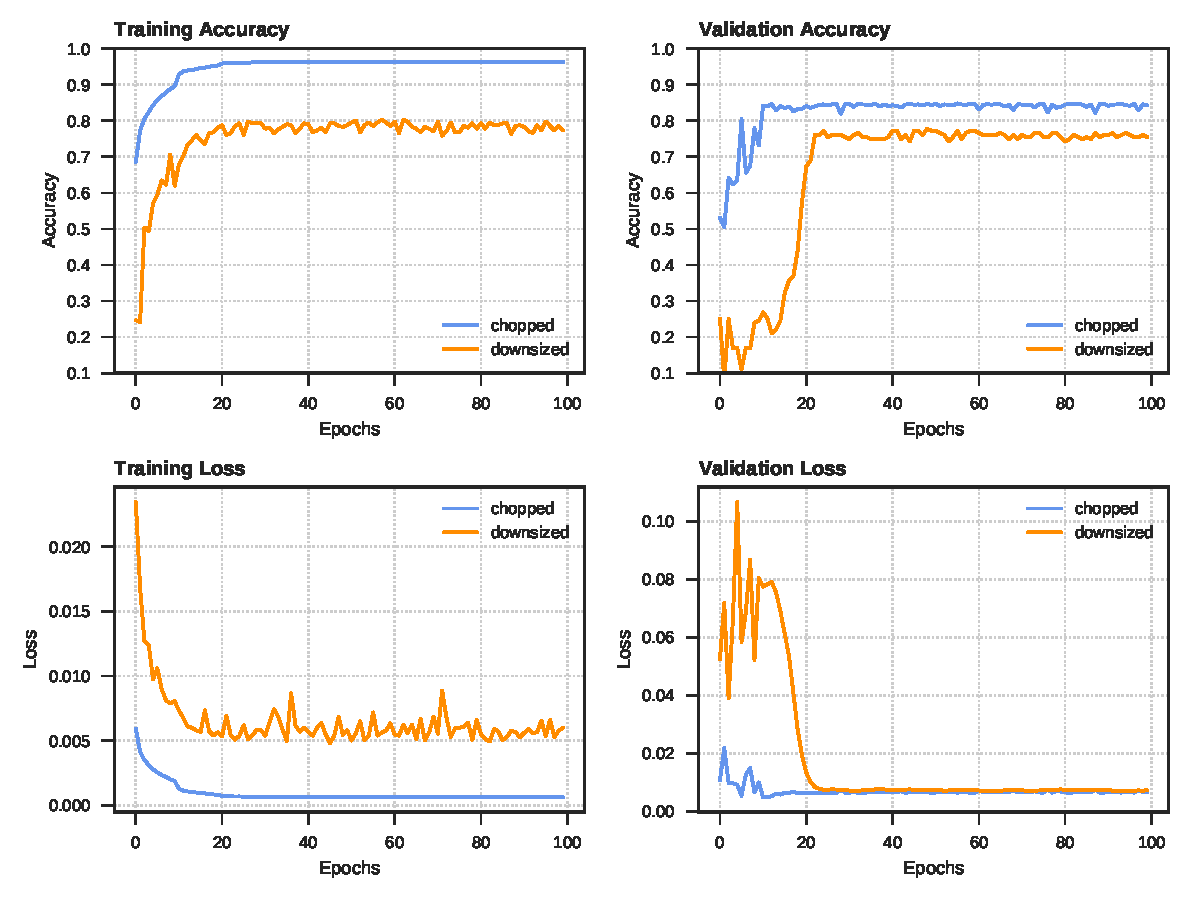
\includegraphics[width=0.8\textwidth]{ch2choppedVsWhole}
    \captionsetup{width=0.8\textwidth}
    \caption[Comparison of whole images vs sub-images]{
Comparison of training ResNet18 model on chopped sub-images vs downsized images from the MDA-MB-231 cell line.
Chopped images were 300$\times$300 crops centred on nuclei.
Whole images were 2160$\times$2160 images downsized to 300$\times$300 pixels.
}
    \label{figure:nn_chopped_vs_whole_curves}
\end{figure}


It should be noted that the validation accuracy reported from the sub-image trained model is for classifying individual sub-images.
One way to better use these individual sub-image classifications is to predict the parent image class based on a consensus of the predicted classes of the child sub-images.
Using this consensus prediction, the sub-image validation classification accuracy increased from 0.847 to 0.912.
Looking at confusion matrices calculated for both sub-image and whole images revealed that neither approach had difficulties at predicting a particular MoA class (figure \ref{figure:nn_chopped_vs_whole_cm}).


\begin{figure}
    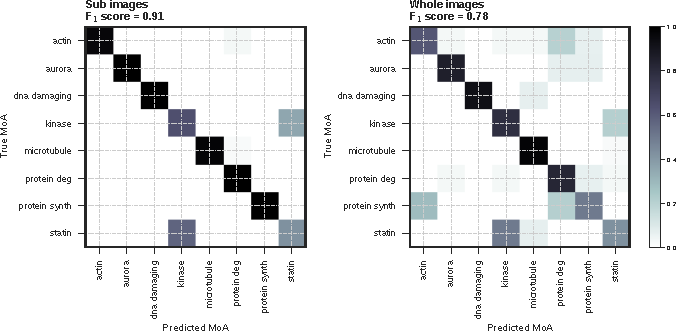
\includegraphics[width=0.8\textwidth]{ch2choppedWholeCM}
    \captionsetup{width=0.8\textwidth}
    \caption[Sub image and whole image confusion matrices]{
Confusion matrices comparing sub-image and whole image classification accuracy on 8 mechanistic classes of compounds with the MDA-MB-231 cell-line.
}
    \label{figure:nn_chopped_vs_whole_cm}
\end{figure}

Following these results the rest of the work involving CNNs used sub-images during training and prediction.
Whilst sub-images improved model training and classification accuracy, it also introduces more complexity as images have to pre-processed to identify cells and crop to a bounding box.
It also introduces another parameter in terms of image size which has to be considered and optimised.
While here I chose 300$\times$300 pixel images corresponding to 97.5 $\mu$m$^2$, this was chosen pragmatically to fully capture a single cell and a portion of any adjacent cells.
This value could be optimised by running several models with differently sized cropped images, although this value is largely dependent on cell line characteristics, magnification and image binning.


\subsection{More complex CNN architectures outperform simpler AlexNet}
As CNNs can be constructed with a wide variety of architectures, and the field is still rapidly developing, I remained close to well established architectures in the literature.
However, as most images are digitally represented in three colour channels (red, green, blue (RGB)), the vast majority of CNN models are constructed in a way that input is restricted to three colour channels, therefore it is necessary to adapt these architectures to work with the differently shaped inputs and additional parameters generated by the 5 channel images generated with the ImageXpress.

The two different CNN architectures were tested based on the hypothesis that a deeper, more complex architecture (ResNet18 \cite{He2015}) will be capable of learning more subtle features, although more complex models with greater numbers of internal parameters are more prone to overfitting when training data is limited.
On the other hand, a more simple model such as AlexNet \cite{Krizhevsky2012} which contains fewer convolutional layers will be less able to perform complex transformations of the data, and therefore theoretically limit the subtle features which can be extracted and learned from an image.
While this might theoretically reduce accuracy, in the absence of large amount of training data it may reduce overfitting due to the fewer number of parameters.

In an effort to reduce over-fitting, both models were evaluated with and without dropout in their dense layers during training.
Dropout is a form of regularisation and works by randomly ignoring a fixed proportion of neurons during the training phase, with the theory that this prevents the model becoming too dependent on the output of a particular neuron and leads to more robust features used for classification.

\begin{figure}
    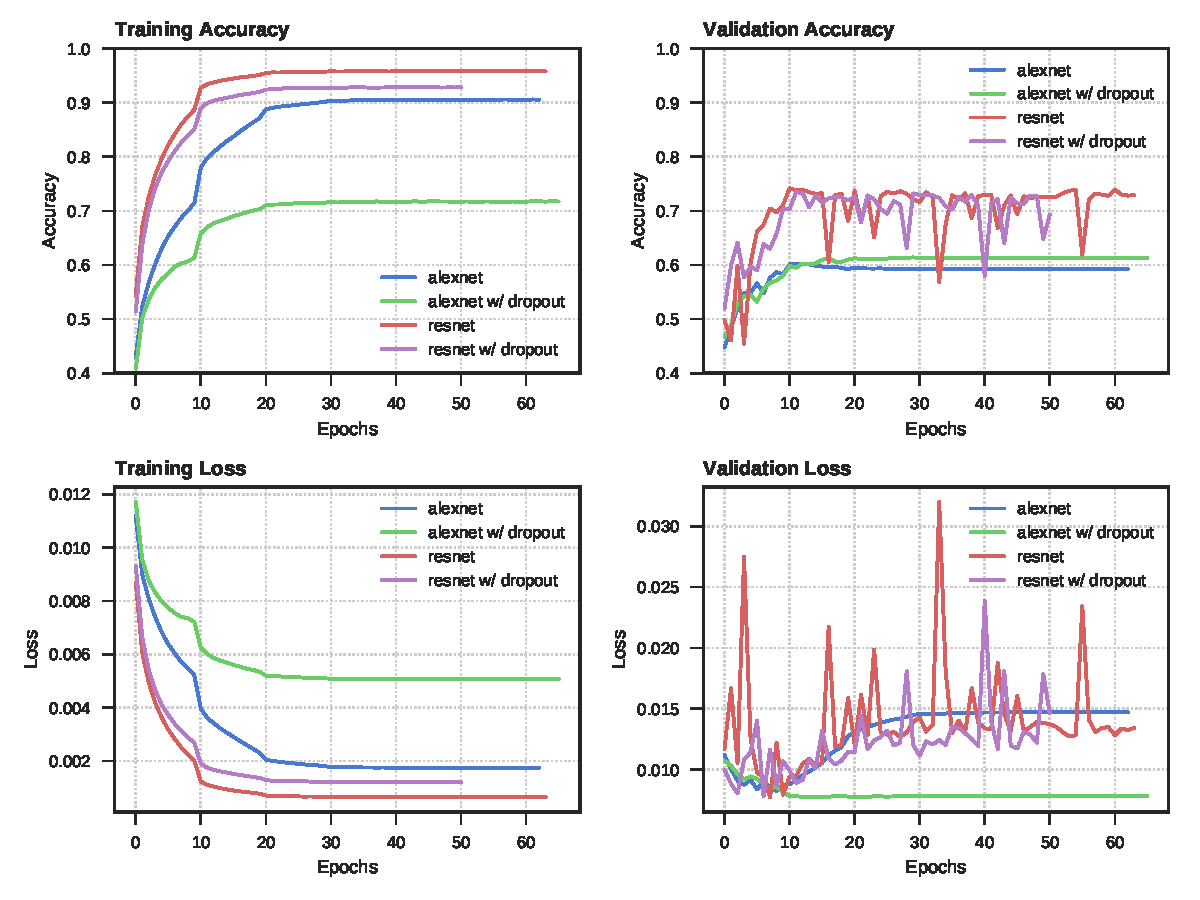
\includegraphics[width=0.8\textwidth]{ch2arch}
    \captionsetup{width=0.8\textwidth}
    \caption[Comparison of CNN architectures]{
Comparison of CNN architectures.
A comparison of AlexNet and ResNet18 architectures with and without dropout training and predicting on 5 channel 244$\times$244 pixel 5 channel images of all eight cell lines.
Loss was calculated using cross entropy on 8 mechanistic classes of compounds.}
    \label{figure:nn_arch}
\end{figure}

Four models in total were trained on sub-images of all eight cell-lines pooled into a single dataset.
The models were ResNet18, ResNet18 with dropout, AlexNet and AlexNet with dropout.
During training the two ResNet18 models outperformed the AlexNets in both training and validation accuracy (figure (\ref{figure:nn_arch})).
AlexNet with dropout layers did outperform the other three approaches when it came to validation loss, as loss did not increase even after many epochs this model demonstrated it is less liable to overfit data.
However, the ResNet18 models showed a substantial increase in classification accuracy, and if training is limited to fewer than 10 epochs they do not show worse over-fitting compared to the AlexNet models.
Additional dropout layers does not seem to reduce ResNet18's liability to overfit beyond 10 epochs, this is not too surprising as the principal behind ResNet18's residual architecture is to limit overfitting, and adding additional dropout to the final fully-connected layers is a crude approach.



\subsection{Standardising image intensity does not improve CNN model convergence}

When training CNN models it is common practice to standardise image intensities.
This pre-processing step consists of subtracting the mean of the image (or image batch) from each pixel and dividing the result by the standard deviation.
The theory is this reduces training time and helps CNN models converge faster by ensuring the weights calculated during training are all on a similar scale which in turn restrains the gradients used in backpropagation.
This pre-processing makes sense in the classical and traditional academic use of CNNs which are often trained on images or photographs from many different sources with inconsistent lighting and colours.
However, the images used in this high-content screening dataset are all from a single microscope with a carefully controlled light source, in addition the intensities of the different channels carry a biological information relating to the abundance of different proteins or cellular structures.
Therefore I wanted to assess if standardising image intensities per image channel improved model convergence and classification accuracy compared to un-normalised intensity values
\footnote{Although un-normalised, intensity values were converted from 16 bit unsigned integers (65536 grayscale values) to 8 bit unsigned integers (256 grayscale values).
This reduces training time and storage size at the expense of intensity accuracy.}.


\begin{figure}
    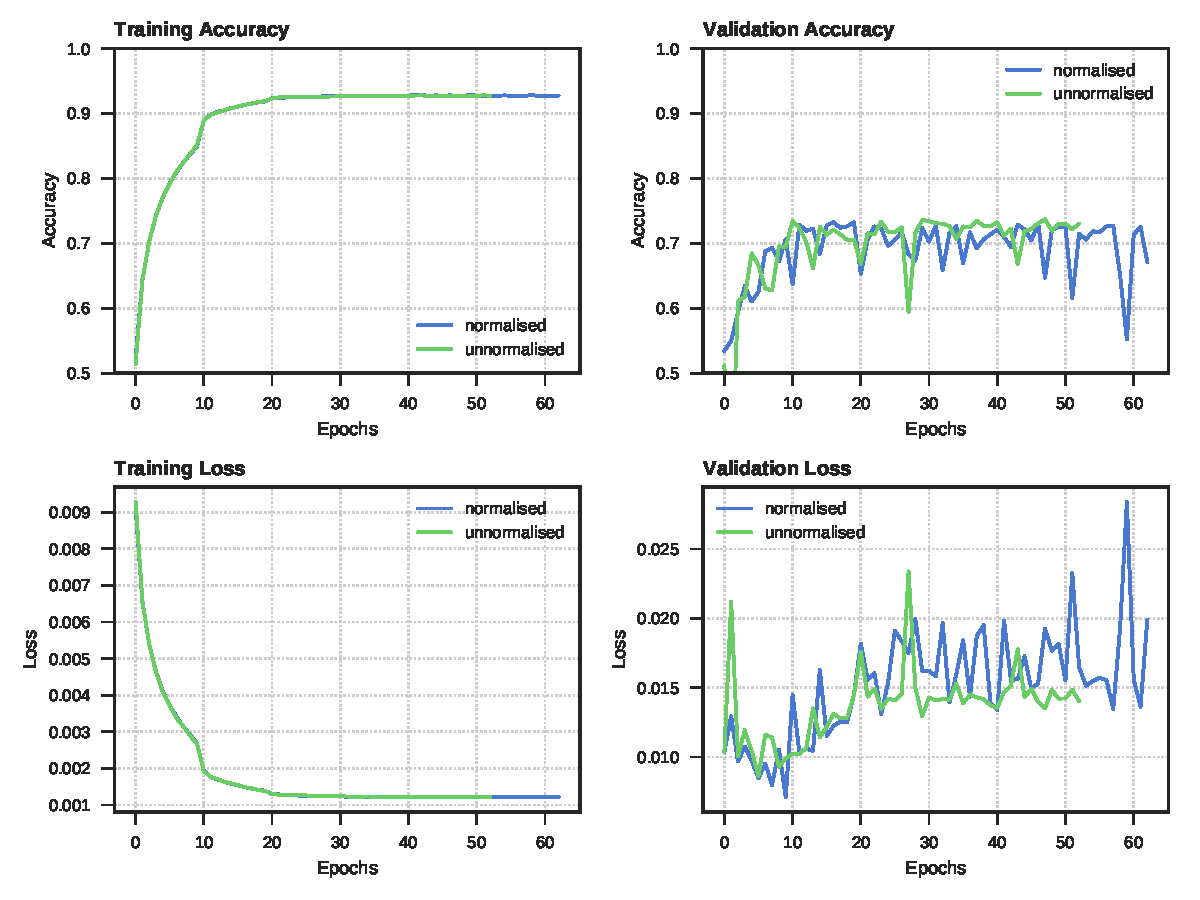
\includegraphics[width=0.8\textwidth]{ch2imgNorm}
    \captionsetup{width=0.8\textwidth}
    \caption[Effect of image intensity normalisation on CNN training]{Effect of image intensity normalisation on CNN training. ResNet18 models training and predicting on eight pooled cell-lines with and without standardising image intensities per image per channel.}
    \label{figure:img_norm}
\end{figure}


Two models based on the ResNet18 architecture were trained on chopped 300$\times$300 pixel images of a pooled dataset of all eight cell lines, one of the models was fed images standardised per channel, the other raw image intensities.
After 48 hours of training (54 and 64 epochs for unnormalised and normalised models respectively \footnote{The number of epochs per 48 hours does not indicate how fast a model converges, but rather the affect of availability of compute resources used for image loading.}) both models demonstrated identical training curves for training accuracy and loss, while validation accuracy and loss curves showed no striking difference in the performance between the two methods, although the normalisation pre-processing step appears to cause sudden drops in model performance indicated by decreased accuracy and increased loss (figure \ref{figure:img_norm}).

There is the possibility that training a model on disparate imaging datasets -- from either different microscopes with different illumination settings, or different concentrations of reagents -- then image standardisation may play a more important role.
However, as intensity standardisation did not improve model performance in this case I chose to continue CNN work using un-standardised images, as there is an argument that standardisation may remove biologically relevant information for no benefit.


\subsection{Single cell/Image aggregates improve classification accuracies with decision trees.}
TODO, delete as appopriate when results come in.

\subsection{Principal component analysis does (not) improve classification accuracy with decision trees.}
TODO, delete as appopriate when results come in.

\subsection{CNN and random forest show equivalent performance at predicting MoA on a single cell-line}

\begin{figure}
    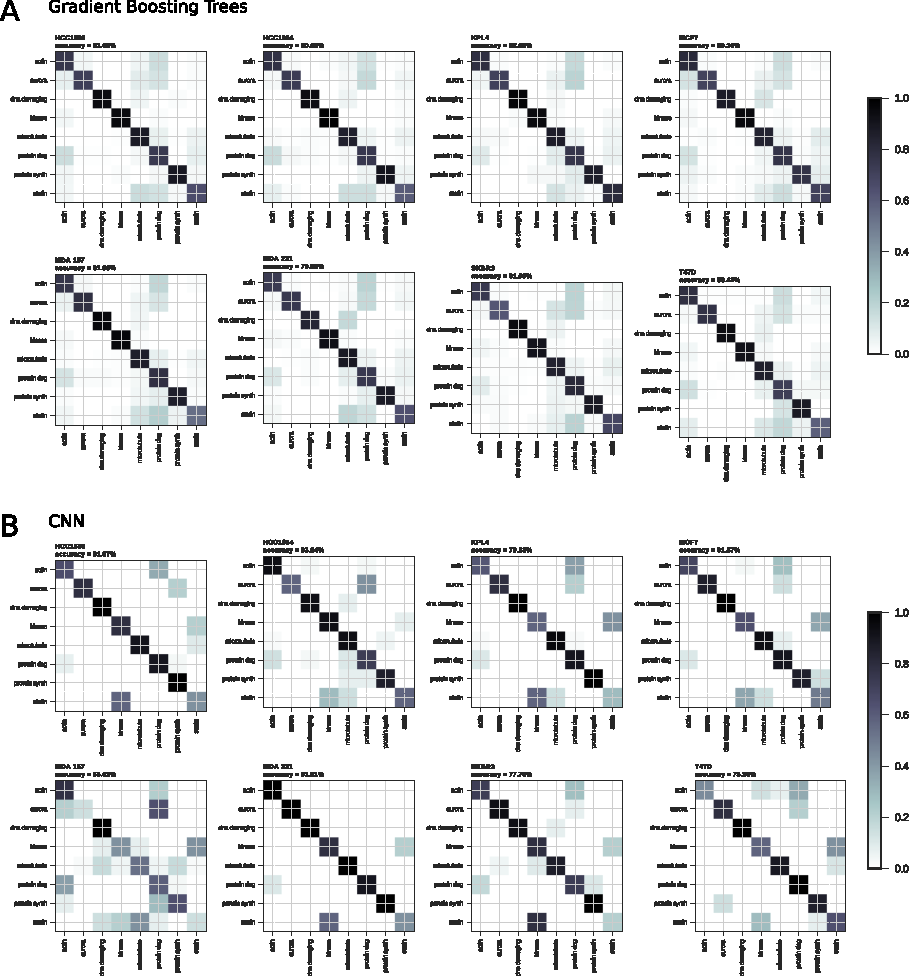
\includegraphics[width=1.0\textwidth]{ch2SingleCellLine}
    \captionsetup{width=0.8\textwidth}
    \caption[Classifying MoA on a single cell-line]{Comparison of ensemble based tree classifier and CNN at predicting compound MoA when trained on tested on an individual cell-line.
    \textbf{(A)} Gradient Boosting tree classifier.
    \textbf{(B)} ResNet18 CNN classifier.
Accuracy measured as the Jaccard similarity score.
    }
    \label{figure:single_cell_line}
\end{figure}


\subsection{Additional data from more cell lines does necessarily improve model performance}

\begin{figure}
    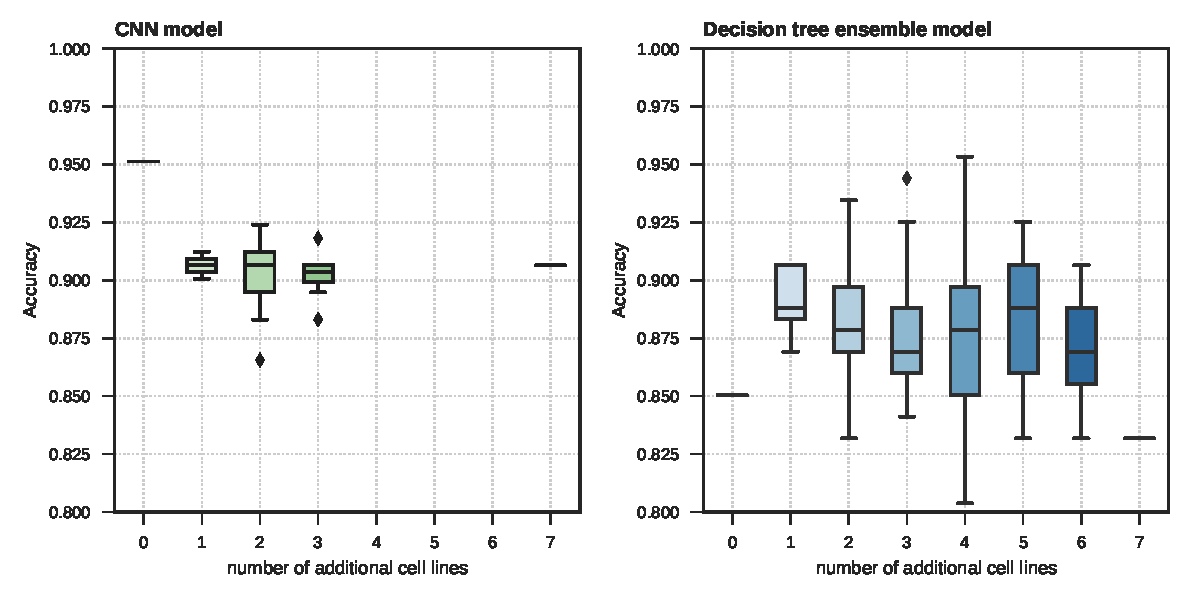
\includegraphics[width=1.0\textwidth]{ch2CumulativeTraining}
    \captionsetup{width=0.8\textwidth}
    \caption[The effect of using additional cell-lines during model training]{
        The effect of using additional cell-lines during model model training.
        Models accuracy when tested on a with-held proportion of MDA-MB-231 data.
        Boxplots show accuracy when tested on different combinations of additional cell-lines.
    }
    \label{figure:cumulative_training}
\end{figure}



\subsection{On the transferrability of classifiers applied to unseen cell lines}

\begin{figure}
    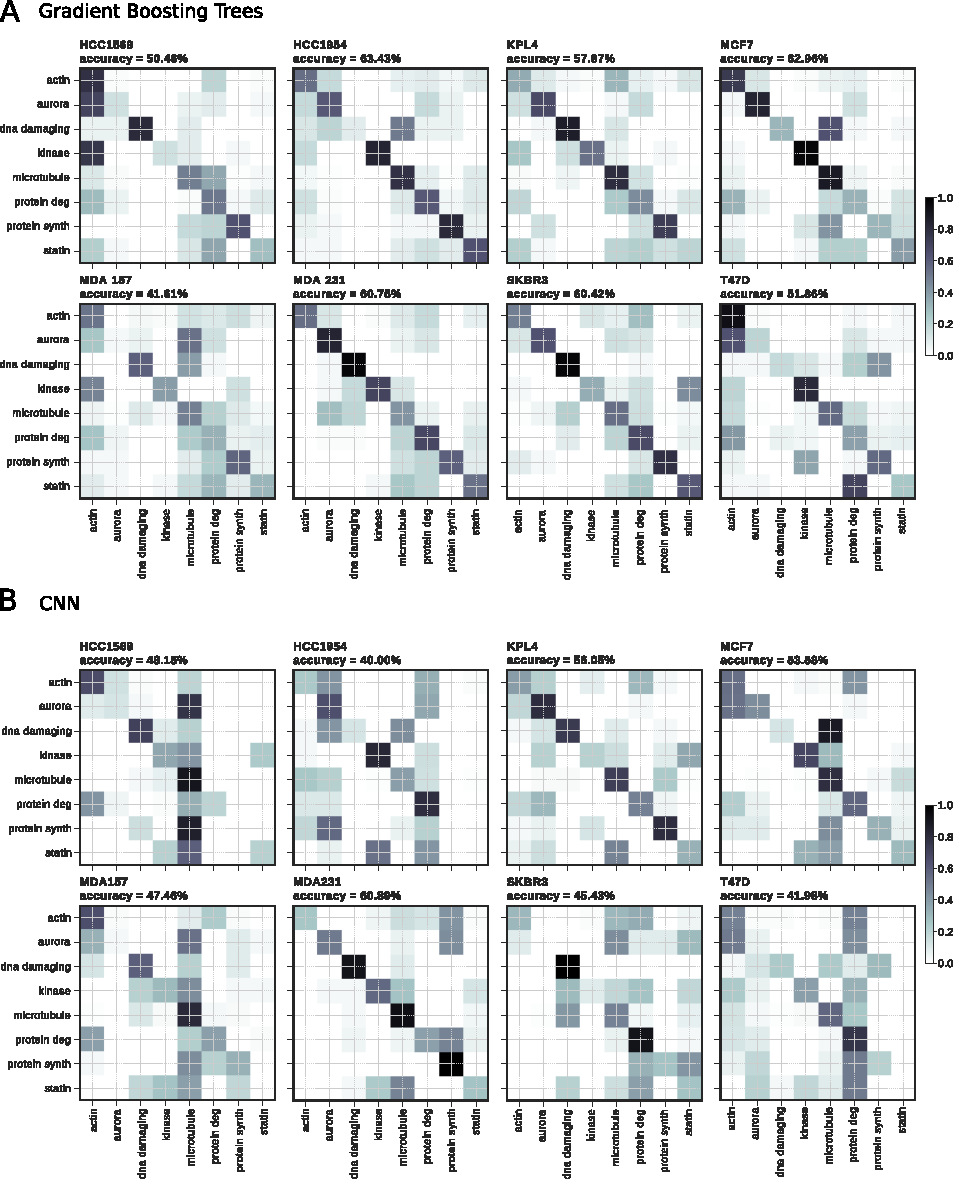
\includegraphics[width=1.1\textwidth]{ch2TransferLearning}
    \captionsetup{width=0.8\textwidth}
    \caption[Confusion matrices of classifiers when applied to unseen cell-lines]{
    Confusion matrices of classifiers applied to unseen cell-lines.
    Models were trained on 7 out of the eight cell-lines and tested on the with-held cell-line (named above confusion matrix).
    }
    \label{figure:transfer_learning}
\end{figure}


%%%%%%%%%%%%%%%%%%%%%%%%%%%%%%%%%%%%%%%%%%%%%%%%%%%%%%%%%%%%%%%%%%%%%%
% DISCUSSION
%%%%%%%%%%%%%%%%%%%%%%%%%%%%%%%%%%%%%%%%%%%%%%%%%%%%%%%%%%%%%%%%%%%%%%

\section{Discussion}
TODO.








%%%%%%%%%%%%%%%%%%%%%%%%%%%%%%%%%%%%%%%%%%%%%%%%%%%%%%%%%%%%%%%%%%%%%%
% METHODS
%%%%%%%%%%%%%%%%%%%%%%%%%%%%%%%%%%%%%%%%%%%%%%%%%%%%%%%%%%%%%%%%%%%%%%


\section{Methods}

\section{Dataset}
The imaging dataset used in this work is the same as in chapter \ref{chapter:tccs}.
For each compound data were used for three concentrations (0.1 $\mu$M, 0.3 $\mu$M, 1.0 $\mu$M).


\subsection{Accuracy}
Validation accuracy during training was measured using the Jaccard similarity score of the $_i$th samples with true label set $y_i$ and predicted label set $\hat{y_i}$:

\begin{equation}
    J(y_i, \hat{y_i}) = \frac{|y_i \cap \hat{y_i}|}{|y_i \cup \hat{y_i}|}
\end{equation}

The F$_1$ score was used post training to determine classification accuracy.
The F$_1$ score is the harmonic mean of both the precision and recall.
So given true positives ($\text{tp}$), false positives ($\text{fp}$) and false negatives ($\text{fn}$):

\begin{align}
        \text{precision} &= \frac{ \text{tp} }{ \text{tp} + \text{fp} } \\
        \text{recall} &= \frac{\text{tp}}{\text{tp} + \text{fn}} \\
        \intertext{the F$_1$ score can be calculated as:}
        F_1 &= 2 \times \frac{\text{precision} \times \text{recall}}{\text{precision} + \text{recall}}.
\end{align}

\subsection{Ensemble of decision trees}
Models were created using scikit-learn version 0.19 in python 3.6.2.
% model
% parameters, grid search of parameters, table of final parameters.
% training, test, train, validation etc.

\subsection{Convolutional neural networks}


All code related to neural networks was written in pytorch v0.3 for python 3.5, and all ANN models were trained on nvidia K80 GPUs.

\subsubsection{Data parallelism}
As training CNNs is computationally expensive and time consuming, data parallelism was used to share batches of images across multiple GPUs trained in parallel.
This technique replicates the CNN model on each device, which processes a portion of the input data, the updated weights for all devices are then averaged and model replicates are updated synchronously after each batch (figure \ref{figure:multi_GPU}).
This speeds up model training approximately linearly with the number of GPUs and allows use of larger batch sizes.

\begin{figure}
    \captionsetup{width=0.8\textwidth}
    \caption[Multi-GPU distributed training]{Increased training speed by data parallelism. Models are replicated across an array of GPUs, the input batch is split evenly among the devices, with each device processing a portion in parallel.
During backpropagation the updated weights for all replicas are averaged and models weights are updated synchronously.}
    \input{figs/ch2MultiGPU.pdf_tex}
    \label{figure:multi_GPU}
\end{figure}

\subsubsection{Architecture}
% describe ResNet18 and AlexNet
% how original architecture was modified to work with 5 channel tensors
% where dropout layers were added, how much dropout


\subsubsection{Training parameters}
% data loaders, image rotation,  how image normalisation was implemented

% image intensity standardisation
Image intensities were standardised on an individual image and channel basis by taking each image in the form of an array [width $\times$ height $\times$ channel] and subtracting the mean of each channel from each pixel value in that channel, and dividing the pixel value by the standard deviation of the original channel.

Batch sizes during training were kept at 64 images.
In the case of using GPU arrays then this was multiplied by the number of GPUs.
Learning rate was set to $1e^{-3}$ decreasing 10-fold every 10 epochs (figure \ref{figure:learningRate}).
Decay was used to aid gradient descent and model convergence.
Models were trained for 100 epochs or 48 hours, whichever was reached first, with model checkpoints every epoch there was an increase maximum validation accuracy.
The optimiser used was ADAM \cite{Kingma2014} with the categorical cross entropy loss function.
%TODO better define what ADAM is

\begin{figure}
    \captionsetup{width=0.8\textwidth}
    \caption[CNN learning rate and decay]{
Learning rate and decay for training CNN models, initialised at $1e^{-3}$ and reduced 10-fold every 10 epochs.
}
    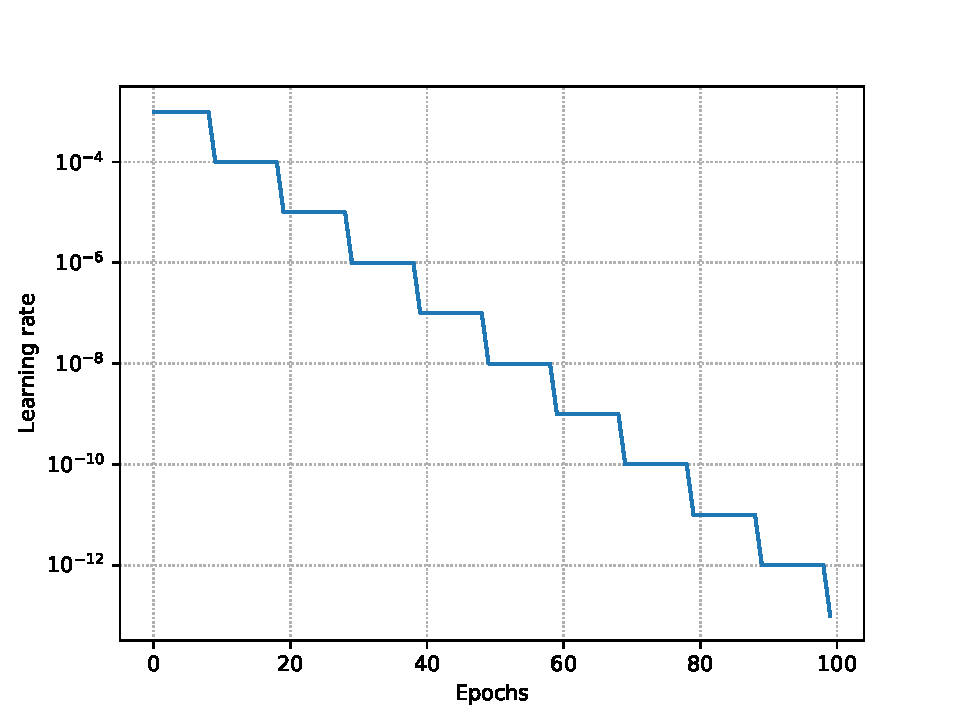
\includegraphics[width=0.5\textwidth]{ch2learningRate}
    \label{figure:learningRate}
\end{figure}


\subsubsection{Image preparation}
% number of images
% encoding
% image chopping

%\printbibliography
\end{document}
